% REVISÃO DE LITERATURA--------------------------------------------------------

\chapter{FUNDAMENTAÇÃO TEÓRICA}
\label{chap:fundamentacaoTeorica}

Capítulo que apresenta o embasamento do tema e os principais tópicos envolvidos na fundamentação teórica desta proposta.

\section{TESTE DE SOFTWARE}

Segundo \cite[p.~144]{SOMMER2011} teste de software é \textit{“destinado a mostrar que um programa faz o que é proposto a fazer e para descobrir os defeitos do programa antes do uso”}.

Testar um software é verificar se o seu comportamento está de acordo com o que foi proposto. Na prática, é o processo de executar um programa de forma que demonstre ao desenvolvedor e ao cliente que ele atingiu seus requisitos especificados, demonstrando que o software funciona corretamente nos cenários para o qual foi projetado \cite{SOMMER2011}.

A principal proposta do teste de software é analisar o resultado de um conjunto de entradas e saídas que serão processadas pelo sistema em forma de uma "caixa-preta"\footnote{Teste de software para verificar a saída dos dados usando entradas de vários tipos através da interface do sistema, o funcionamento interno do sistema é desconhecido.}, e gerar um conjunto de dados de saída do processo de transformação. Os resultados são os testes de validação e testes de defeito. O teste de validação visa garantir que o sistema execute corretamente um determinado caso de teste que reflete o uso rotineiro do sistema. O teste de defeito revela erros no processo interno do sistema onde o sistema executa entradas incorretas gerando saídas imprecisas ou obscuras. Sommerville (2011) ilustra um modelo que resume essa ideia na Figura \ref{modeloEntradaSaida}.  

\begin{figure}[h!]
	\centering
	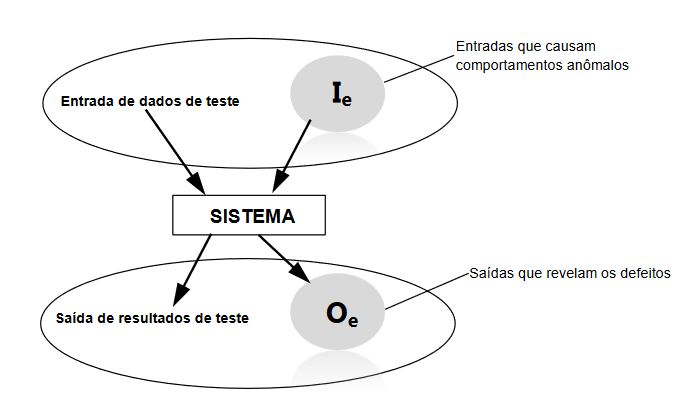
\includegraphics[scale=0.7]{dados/figuras/modelo_entradaSaida.JPG}
	\caption{Um modelo de entrada-saída de teste de programa.}
	Fonte: \cite[p.~145]{SOMMER2011}
	\label{modeloEntradaSaida}
\end{figure}


A Figura \ref{modeloEntradaSaida} apresenta um conjunto de entradas, representadas pelo conjunto \textbf{I}(\textit{input}) que serão processadas pelos sistema a ser testado, entre as entradas do conjunto contém um subconjunto \textbf{Ie} que representa um conjunto de entradas imprecisas e erradas, este conjunto de dados pode causar um erro ou apresentar um defeito de sistema. Então uma bateria de testes é realizada a partir das entradas especificadas gerando o conjunto de saídas \textbf{O}(\textit{output}), alguns dos testes devem apresentar erro pois representam o conjunto de saídas de \textbf{Oe} que é resultante da entrada de \textbf{Ie}. O objetivo dos conjuntos de entradas e saídas de testes e avaliação dos requisitos, já os subconjuntos testam a segurança a falhas e defeitos do sistema.

O teste é apenas parte de um processo de validação e verificação, proporcionando uma etapa importante dentro do processo de desenvolvimento, mas erros podem vir a acontecer, eles não demonstram que o software é livre de falhas, e que ele irá se comportar como o planejado no ambiente para qual foi projetado. É possível que o teste que não foi projetado seja aquele que descobriria uma falha no sistema \cite{SOMMER2011}.

Uma boa estratégia para teste de software é a de aplicação de testes de: baixo nível para verificar se um trecho de código foi implementado corretamente (teste de unidade), testes de integração que verificam a funcionalidade de um componente e a sua incorporação com outros componentes na arquitetura de software; teste de validação que demonstra se os requisitos foram atendidos, e o teste de sistema que aprova o software quando ele é incorporado em sistemas maiores. Cada etapa é realizada com uma serie de técnicas que auxiliam na resolução de problemas e detecção de falhas \cite{PRESMA2016}.

A estratégia de testes pode ser entendida como um espiral, partindo do centro para a sua extremidade passando pelas fases de teste de unidade, integração, validação e sistema. A FIGURA \ref{espiral} mostra a ideia proposta por Pressman.

\begin{figure}[h!]
	\centering
	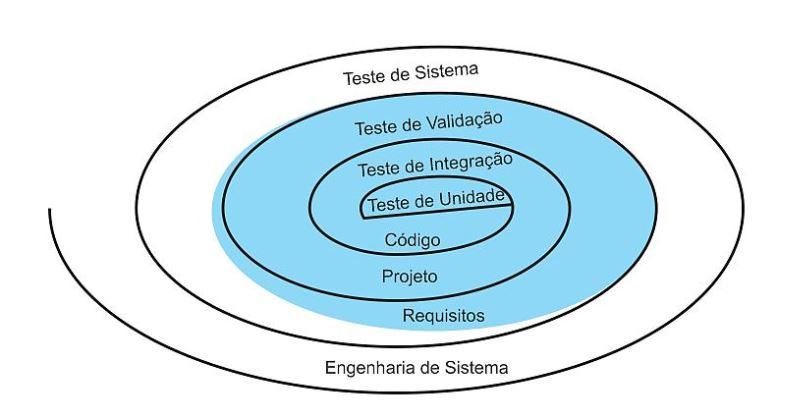
\includegraphics[scale=0.6]{dados/figuras/espiralPres.JPG}
	\caption{Estratégia de teste.}
	Fonte: \cite[p.~470]{PRESMA2016}
	\label{espiral}
\end{figure}

Os testes unitários estão no centro da espiral e representam os fragmentos de código a menor parte de um requisito. Funções\footnote{Conjunto de comandos que realiza uma tarefa específica em um módulo dependente de código.}, classes\footnote{Descrição que abstrai um conjunto de objetos com características similares} e variáveis\footnote{Um objeto (uma posição, frequentemente localizada na memória) capaz de reter e representar um valor ou expressão. } são testados nessa etapa. Conforme se avança na espiral se dá início ao teste de integração de componentes, esta etapa trata de verificar se a integração de diferentes fragmentos do software e suas interfaces\footnote{Recurso que permite a elaboração de códigos flexíveis, diminuindo a amarração do código, permitindo o acesso a atributos e métodos de outras classe sem acessar esta classe diretamente.} não acarretam problemas em funcionalidades já testadas. Seguindo na espiral a validação, já mencionada, trata de validar os requisitos do sistema. Por fim o teste de sistema consiste em validar se todos os componentes integrados e validados se combinam para formar um único produto de software que pode integrar sistemas maiores.

 O processo de teste pode atender várias outras etapas do processo de produção de um software afim de garantir maior qualidade no produto final. De maneira geral os testes podem rastrear defeitos no programa, mas isso não impede que existam defeitos remanescentes \cite{SOMMER2011}.

\subsection{Teste Unitário}

Teste de unidade é o processo que foca nas menores unidades do software, como métodos, classes e variáveis. Neste processo pode-se usar como guia a descrição do projeto para se testar caminhos de controle importantes, e descobrir falhas nos limites dos módulos \cite{PRESMA2016}.

No teste orientado a objetos\footnote{Paradigma de programação baseado no conceito de "objetos", que podem conter dados na forma de campos, também conhecidos como atributos, e códigos, na forma de procedimentos, também conhecidos como métodos.}, devem-se cobrir todas as características  do objeto de modo que todas as operações associadas devem ser testadas. Todos os atributos associados ao objetos devem ser definidos e verificados, e todos os eventos que causam alteração no objeto devem ser testada colocando o objeto em todos os estados possíveis \cite{SOMMER2011}.

O teste de unidade foca em tarefas importantes de um módulo, tais como interface de comunicação, estrutura de dados locais, condições limites, caminhos independentes e caminhos de manipulação de erro, como no esquema da FIGURA \ref{unidade} ilustrada por Pressman.

\begin{figure}[H]
	\centering
	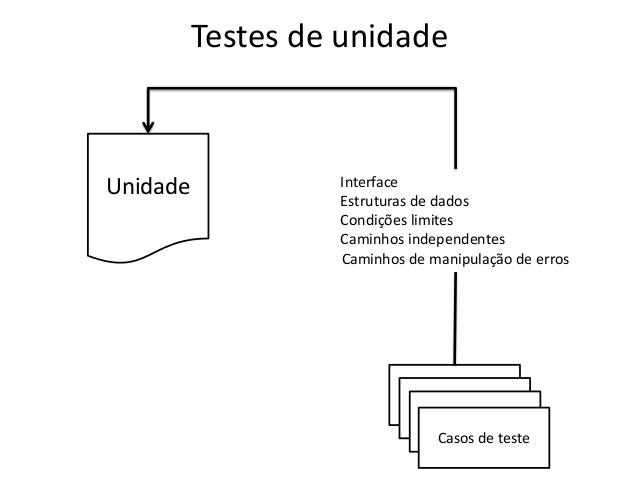
\includegraphics[scale=0.5]{dados/figuras/testeDeUnidade.jpg}
	\caption{Teste de Unidade.}
	Fonte: \cite[p.~474]{PRESMA2016}
	\label{unidade}
\end{figure}

A Figura \ref{unidade} considera os principais objetivos do teste de unidade. O teste de interface do módulo é responsável por testar a comunicação deste módulo com os demais módulos e se o fluxo de dados que percorre a interface entra e sai corretamente, se o fluxo de entrada e saída forem incorretos todos os outros testes irão falhar. A estrutura de dados deve ser testada para garantir que os dados armazenados pelo módulo permaneçam íntegros durante todo o processo de execução do algoritmo. Os valores e condições limites devem ser testados para garantir que o software possa operar nos extremos de sua especificação mantendo a integridade e sua capacidade de processamento. Por fim os testes de manipulação de erro são testados para garantir que uma exceção ou uma falha é tratada e corrigida pelo software \cite{PRESMA2016}.

Teste unitários sempre que possível devem ser automatizados, para quando a aplicação sofrer alguma alteração ou for integrada a um outro componente, os testes possam ser realizados novamente. O uso de \textit{Framework}\footnote{Plataforma de desenvolvimento que contém uma estrutura base para desenvolvimento de soluções em projetos de software.} de automação facilita este processo, como o \textit{JUnit}. Por muitas vezes o objeto que será testado possui dependências em outros objetos que ainda não foram implementados ou não estão disponíveis no ambiente, para o que o processo de teste não atrase é possível a utilização de \textit{Framework} do tipo \textit{mock objects} que simula o comportamento de objetos externos através métodos simulados \cite{SOMMER2011}. 



\subsection{Teste de Componente/Integração}

Os componentes em softwares são compostos de diversos objetos que interagem. Os testes em componentes compostos devem focar nas interfaces de comunicação. Deve-se garantir que quando objetos diferentes são integrados eles se comuniquem de acordo com o especificado. Os testes de unidade não cobrem os testes de componente pois avaliam a interação de um único objeto, já os testes de componente avaliam a interação de diversos componente pelas suas interfaces, o que pode gerar comportamento anômalos dos objetos já testados \cite{SOMMER2011}.


Os testes em interface são os mais difíceis de serem realizados pois problemas podem surgir somente em uma situação inesperada \cite{SOMMER2011}. Dados podem ser perdidos, funções de objetos diferentes combinadas podem não produzir o efeito desejado, estruturas globais podem apresentar problemas, estes entre outros erros podem surgir na integração de componentes \cite{PRESMA2016}.


Os testes unitarios comuns não são muito eficientes em encontrar erros de interface. Inspeções de código e validações de funcionalidades do projeto podem ser mais eficientes para revelar os erros. Inspeções podem se focar no comportamento da interface durante a execução e integração com outros componentes, o comportamento deve ser validado de acordo com a especificação \cite{SOMMER2011}. O objetivo do teste de componente é construir uma estrutura de software baseado em unidades testadas.


 
\subsection{Teste de Validação}

O teste de validação começa quando o teste de componentes termina. O software está em um estado parcialmente acabado onde já é possivel processar entradas e produz saídas. O teste de validação de software se trata de uma série de comparações do produto já implementado com os requisitos propostos no início do desenvolvimento. A validação pode ser definida como a maneira de atingir razoavelmente bem o que foi especificado pelo cliente nos requisitos do software \cite{PRESMA2016}.  


No caso de softwares personalizados para clientes específicos, o teste de validação pode ser realizado pelo cliente juntamente com a equipe de desenvolvimento. O cliente recebe uma versão inacabada do software, ele testa as funcionalidades desenvolvidas até o momento e avalia se os requisitos pedidos foram atendidos. Se o  desvio dos requisitos foram descobertos é criada uma lista de deficiência e deve se estabelecer um método para solucionar os desvios \cite{PRESMA2016}.


\subsection{Teste de Sistema}

A última etapa de teste se foca na interação de componentes para dar início a uma nova versão do sistema, e em seguida é dado início à bateria de testes do sistema integrado. Apesar de se parecer com o teste de componentes, o teste de sistema se preocupa com a interação e comunicação do sistema com outro diversos componentes, software de terceiros, hardware, rede, informação e pessoas. Nesta etapa é testada a comunicação entre os diversos componente, e suas interfaces se são compatíveis, se interagem corretamente e se transferem os dados corretamente no momento certo \cite{SOMMER2011}.


Uma boa estratégia para teste de sistema é criar testes de interação com o sistema baseados em casos de uso. Geralmente cada caso de uso representa uma tarefa mais complexa, o que exige uma série de transações do sistema. Testes de sistema geralmente são mais difíceis de se realizar pois podem produzir saídas muito grandes e de difícil previsão, mais é possível analisar uma saída e verificar sua credibilidade tendo como base uma previsão realizada com antecedência \cite{SOMMER2011}.



\section{JUNIT 5 FRAMEWORK}

O  \textit{JUnit} é uma plataforma de execução de testes na JVM (\textit{Java virtual machine}), que utiliza uma estrutura de anotações para identificar métodos que especificam um teste. A nova arquitetura do \textit{JUnit} 5 é dívida em módulos que são agrupados em três pacotes que compõem o \textit{framework}. 

\begin{itemize}

\item O \textit{JUnit Plataform} contém elementos estruturais para execução de testes. Esta plataforma implementa uma API de \textit{TestEngine}\footnote{Plataforma que permite a execução de testes baseados em JUnit.} possibilitando que outros \textit{frameworks} possam ser executados. Por exemplo, a \textit{TestEngine} possibilita a execução de testes escritos usando o modelo de programação \textit{JUnit Jupiter} \cite{Junit}. 


\item O \textit{JUnit Jupiter} é o modelo de programação e extensão de API utilizado para criação de testes no \textit{JUnit} 5, é neste pacote que estão definidas as anotações e classes que são necessárias para a construção dos testes, como a anotação \textit{@Test} e várias outras \cite{Junit}.


\item O \textit{JUnit Vintage} é um pacote que provê uma \textit{TestEngine} para execução de testes baseados em versões do \textit{JUnit} 3 e \textit{JUnit} 4 da plataforma \cite{Junit}.


\end{itemize}


Cada módulo é distribuído como um artefato\footnote{Um subproduto concreto produzido durante o desenvolvimento de software.} e publicado em diversas plataformas de IDEs (\textit{Integrated development environment}) populares (\textit{IntelliJ IDEA , Eclipse , NetBeans e Visual Studio Code}), e ambientes de construção\footnote{Conjunto de ferramentas criadas para auxiliar a criação e desenvolvimento de um software.} (\textit{Gradle , Maven e Ant}). O \textit{JUnit} 5 requer o Java 8. No entanto, ainda é possível testar o código que foi compilado com versões anteriores do JDK (\textit{Java Development Kit}) \cite{Junit}.


Com o \textit{Junit} é possível criar testes unitários para verificar as funcionalidades de classes e seus métodos. Assim é possível automatizar a execução de todos os testes unitários de forma que quando for criada uma nova versão estável do sistema, o \textit{framework} execute todos os testes unitários para garantir a integridade e estabilidade do sistema desenvolvido.


% \subsection{Adicionando JUnit Usando Maven }

% Para a utilização do \textit{Junit} basta baixar os artefatos desejados a IDE de preferencia ou adicionar as dependências com a ferramenta de gerenciamento de dependências opcional do usuário. A FIGURA \ref{mvn} ilustram a importação\footnote{Recurso que permite amarrar o código de uma classe ou método externo a outras classes.} do pacote \textit{JUnit Jupiter} pela ferramenta de gerenciamento de dependências \textit{Maven}. 

% \begin{figure}[h!]
% 	\centering
% 	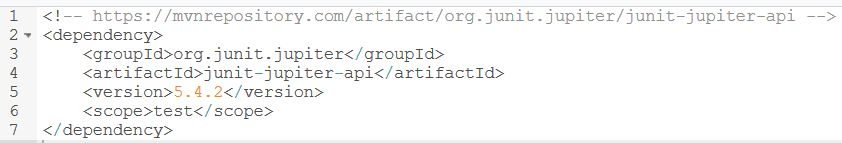
\includegraphics[scale=0.7]{dados/figuras/mvnJu.JPG}
% 	\caption{Importação do Pacote JUnit Jupiter API Utilizando Maven.}
% 	Fonte: \cite[Link:~https://mvnrepository.com/artifact/org.junit.jupiter/junit-jupiter-api/5.4.2]{Maven}
% 	\label{mvn}
% \end{figure}

% A FIGURA \ref{mvn} apresenta a importação do pacote \textit{JUnit Jupiter} onde cada linha tem a sua seguinte função. 

% \begin{itemize}
  
% \item[1]: é indicado o repositório central onde são armazenadas todas as versões do pacote importado. 

% \item[2]: a \textit{tag} \textit{<dependencies>} é aberta, é dentro desta \textit{tag} que cada dependência é definida individualmente, 


% \item[3]: a \textit{tag} \textit{<groupId>} é aberta e fechada, ela é o identificador único do pacote \textit{"org.junit.jupiter”} responsável por indicar a coordenada \textit{Mavem} do projeto.

% \item[4]: a \textit{tag} \textit{<artifactId>} é aberta e fechada, ela é geralmente o nome pelo qual o projeto é conhecido \textit{"junit-jupiter-api"},  ela juntamente com a \textit{tag} \textit{<groupId>} é responsável separar o projeto de todos os outros do repositório central.


% \item[5]: alterações no código geram versões diferentes do mesmo pacotes a \textit{tag} \textit{<version>} \textit{"5.4.2"} indica quais alterações feitas no código e devem ser baixadas.
 
% \item[6]: esta \textit{tag} \textit{<scope>} faz referência ao tipo de trabalho \textit{"test"} que será realizado pelo pacote, e limita a transitividade de um pacote.


% \item[7]: é responsável por fecha a chave de \textit{tags} \textit{<dependency>}.

% \end{itemize}


% Para que a importação seja realizada com sucesso a dependência deve ser declarada em um arquivo de POM.xml (Project Object Model) que contem a lista de dependências do projeto, este é a peça fundamental de um projeto Maven \cite{Maven}.



\subsection{Utilizando JUnit}

O \textit{JUnit} utiliza uma referência por anotações. Essas funcionam como uma estrutura de cascata que define quais elementos devem ser executados e criados antes dos testes terem início. Elas também podem ser usadas como filtro para indicar quais testes devem ser realizados primeiro, caso o processo de teste seja muito extenso e custoso. 
As principais anotações são apresentadas na Tabela \ref{tab:tags1} no site do \textit{JUnit}:


\begin{table}[!h]
\caption[Anotações JUnit]{Anotações JUnit.}
\label{tab:tags1}
\begin{tabular}{|l|l|}
\hline
\textbf{Anotação (Tag)} & \textbf{Descrição}                                                                                                                                           \\ \hline
@Test                   & \begin{tabular}[c]{@{}l@{}}Indica que um método é um método de teste. Ao contrário da \\ anotação @Test do JUnit 4, essa anotação não declara \\ nenhum atributo, já que as extensões de teste no JUnit Jupiter \\ operam com base em suas próprias anotações dedicadas.\end{tabular} \\ \hline
@BeforeEach             & \begin{tabular}[c]{@{}l@{}}Indica que o método anotado deve ser executado antes de \\ cada  método @Test , @RepeatedTest , \\ @ParameterizedTest ou @TestFactory na classe atual\end{tabular}                                                                                         \\ \hline
@AfterEach              & \begin{tabular}[c]{@{}l@{}}Indica que o método anotado deve ser executado após \\ cada método @Test , @RepeatedTest , \\ @ParameterizedTest ou @TestFactory na classe atual\end{tabular}                                                                                              \\ \hline
@TestInstance           & \begin{tabular}[c]{@{}l@{}}Usado para configurar o ciclo de vida da instância de \\ teste para a classe de teste anotada.\end{tabular}                                                                                                                                                \\ \hline
@DisplayName            & \begin{tabular}[c]{@{}l@{}}Declara um nome de exibição personalizado para a classe \\ de teste ou método de teste.\end{tabular}                                                                                                                                                       \\ \hline
@Disabled               & Usado para desabilitar uma classe de teste ou método de teste.                                                                                                                                                                                                                        \\ \hline
@BeforeAll              & \begin{tabular}[c]{@{}l@{}}Indica que o método anotado deve ser executado antes de todos os \\ métodos @Test , @RepeatedTest , @ParameterizedTest e \\ @TestFactory na classe atual.\end{tabular}                                                                                     \\ \hline
@AfterAll               & \begin{tabular}[c]{@{}l@{}}Indica que o método anotado deve ser executado após todos os\\ métodos @Test , @RepeatedTest , @ParameterizedTest e \\ @TestFactory na classe atual.\end{tabular}                                                                                          \\ \hline
\end{tabular}
\\ Fonte: \cite[https:~//junit.org/junit5/docs/current/user-guide/overview]{Junit}
\end{table}

É possível encontrar todas as anotações e suas especificações no pacote \textit{org.junit.jupiter.api} no site oficial do \textit{JUnit}.



A Figura \ref{JUnit} apresenta um teste simples sendo implementado utilizando as ferramentas do \textit{JUnit} : 

\begin{figure}[!h]
	\centering
	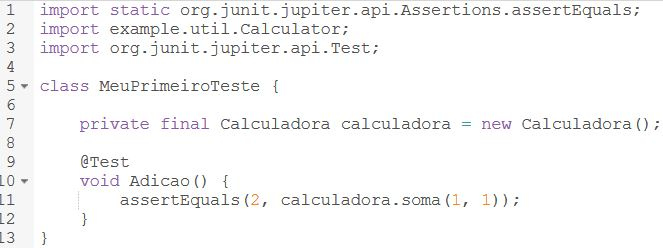
\includegraphics[scale=0.9]{dados/figuras/tesLine.JPG}
	\caption{Teste utilizando JUnit.}
	\label{JUnit}
\end{figure}

O trecho de código da Figura \ref{JUnit} apresenta um teste simples. Na linha 2 é realizada a importação da classe \textit{"Calculadora"}, que se trata de uma classe concreta que implementa o método “soma”, este método recebe dois valores inteiros como parâmetro e retorna a soma dos dois valores.  O restante do código possui as seguintes características:

\begin{itemize}

\item[1]:  é importada a função de \textit{"assertEquals"} do pacote \textit{JUnit}, esta função e responsável por comparar dois valores, o primeiro valor é o valor esperado de uma operação, resultado, ou estado. O segundo valor é o valor resultante da chamada de uma função, classe, ou variável que se deseja testar. 

\item[2]: realiza a importação da classe \textit{"Calculadora"} que será testada. 

\item[3]: realiza a importação do pacote de testes \textit{JUnit} onde se encontram as \textit{tags} de anotações é os metodos\footnote{Determinam o comportamento dos objetos de uma classe e são análogos às funções.} do \textit{Framework}. 

\item[5]: a classe principal \textit{"MeuPrimeiroTeste"} é aberta. 

\item[7]: é instanciado\footnote{Criar um novo objeto do mesmo tipo dessa classe} um objeto do tipo \textit{"Calculadora"} na variável \textit{"calculadora"}. 

\item[9]: é utilizada a anotação \textit{@Test}, esta anotação sinaliza que o método a seguir é um método que deve realizar um teste. 

\item[10]: o método de nome \textit{"Adicao"} é declarado, sendo do tipo \textit{"void"} (sem retorno). 

\item[11]: a função importada \textit{"assertEquals"} é chamada, a ela é passado o valor inteiro 2, e em seguida a função \textit{"calculadora.soma(1,1)"}. A excecução do progama segue com a chamada do metodo  \textit{"soma"} realizada pelo objeto instanciado na variável "calculadora". A função \textit{"soma"} chamada recebe dois valores, realiza a soma e retorna o resultado. O retorno da função \textit{"soma"} é agurdado para comparação com o primeiro valor passado a função \textit{"assertEquals"}.

\item[12]: o método \textit{"Adicao"} é fechado.

\item[13]: a classe principal é fechada.

\end{itemize}

Caso o retorno da função \textit{"soma"} seja um inteiro "2", o mesmo resultado esperado pelo \textit{assertEquals}, o resultado do teste será verdadeiro, então logo o teste é aprovado. Caso a função \textit{"soma"} retorne outro valor diferente de um inteiro "2"  o resultado será falso, logo o teste é reprovado. 


    Mais funções do \textit{Framework JUnit} serão explorados ao longo deste trabalho.


\section{MOCKITO FRAMEWORK}


\textit{Mockito} é um \textit{framework} de simulação baseado em JAVA que é utilizado para testes unitários em aplicativos. Um teste de unidade deve testar a funcionalidade isoladamente. Todos os efeitos colaterais possíveis de outras classes ou do sistema devem ser eliminados para um teste de unidade  \cite{Mockito}. 


O \textit{Mockito} é usado para simular interfaces, de modo que uma funcionalidade fictícia possa ser adicionada a uma interface simulada que pode ser usada no teste de unidade. O objetivo principal é no sentido de que os objetos simulados são criados para imitar objetos reais de maneira controlada. Os objetos simulados são basicamente uma versão simulada do objeto original que é programaticamente\footnote{Que possui um plano de atividade para realizar uma determinada função.} criado para verificar o comportamento de outro objeto. O princípio da programação orientada a objetos é a comunicação e o relacionamento entre objetos, à medida que o contexto se amplia, a unidade individual como um objeto pode ter que ser expandida em módulos. Portanto, quando se testa um componente, é possível testar os módulos como uma unidade individual e seu relacionamento, o ponto é que um objeto individual raramente faz sentido em um programa. Objetos funcionam em relação. Assim, escolher uma unidade para testar é tão necessário quanto testar seu relacionamento. O objeto \textit{mocking} é uma técnica para testar unidades isoladamente, simulando suas unidades dependentes.


% \subsection{Adicionando Mockito Usando Maven}

% Para a utilização do \textit{Mockito} basta baixar os artefatos desejados a IDE de preferencia ou adicionar as dependências com a ferramenta de gerenciamento de dependências opcional do usuário. A FIGURA \ref{mvn2} ilustram a importação do pacote \textit{Mockito 2.0.2-beta} pela ferramenta de gerenciamento de dependências \textit{Maven}. 

% \begin{figure}[H]
% 	\centering
% 	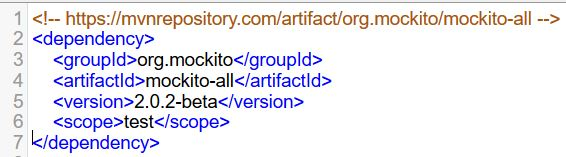
\includegraphics[]{dados/figuras/mockito.JPG}
% 	\caption{Importação do Pacote Mockito 2.0.2-beta Utilizando Maven.}
% 	Fonte: \cite[https:~//mvnrepository.com/artifact/org.mockito/mockito-all/2.0.2-beta]{Maven}
% 	\label{mvn2}
% \end{figure}

% A FIGURA \ref{mvn2} apresenta a importação do pacote \textit{Mockito 2.0.2-beta} onde cada linha e tem a sua seguinte função: 

% \begin{itemize}
  
% \item[1]: é indicado o repositório central onde são armazenadas todas as versões do pacote importado. 

% \item[2]: a \textit{tag} \textit{<dependencies>} é aberta, é dentro desta \textit{tag} que cada dependência é definida individualmente, 

% \item[3]: a \textit{tag} \textit{<groupId>} é aberta e fechada, ela é o identificador único do pacote \textit{"org.mockito”} responsável por indicar a coordenada \textit{Mavem} do projeto.

% \item[4]: a \textit{tag} \textit{<artifactId>} é aberta e fechada, ela é geralmente o nome pelo qual o projeto é conhecido \textit{"mockito-all"},  ela juntamente com a \textit{tag} \textit{<groupId>} é responsável separar o projeto de todos os outros do repositório central.


% \item[5]: alterações no código geram versões diferentes do mesmo pacotes a \textit{tag} \textit{<version>} \textit{"2.0.2-beta"} indica quais alterações feitas no código e devem ser baixadas.
 
% \item[6]: esta \textit{tag} \textit{<scope>} faz referência ao tipo de trabalho \textit{"test"} que será realizado pelo pacote, e limita a transitividade de um pacote.


% \item[7]: é responsável por fecha a chave de \textit{tags} \textit{<dependency>}.

% \end{itemize}


% Para que a importação seja realizada com sucesso a dependência deve ser declarada em um arquivo de \textit{POM.xml (Project Object Model)} que contem a lista de dependências do projeto, este é a peça fundamental de um projeto \textit{Maven} \cite{Maven}.



\subsection{Utilizando Mockito}

O \textit{Mockito} permite a utilização de vários métodos para a criação de objetos simulados, desde \textit{tags} de anotações a métodos estáticos. 
Na utilização de \textit{tags} de anotação como \textit{@Mock}, é necessário que se defina o comportamento dos objetos anotados e em seguida invoque o método \textit{MockitoAnnotations.initMocks(this)} para preencher os campos anotados.
Na utilização de métodos estáticos, adicionando o \textit{org.mockito.Mockito.*;} é possível trabalhar com importação estática e utilizar os métodos do pacote \textit{mockito} diretamente nos testes. As importações estáticas permitem que membros estáticos sejam chamados, isto é, métodos e campos de uma classe podem ser chamados diretamente \cite{Mockito}, \cite{Javadoc}.
 A FIGURA \ref{mockito} é um exemplo de teste utilizando importação estática do pacote \textit{Mockito}.




A FIGURA \ref{mockito} traz na linha de código 8 a classe \textit{Calculadora}. Esta classe se trata de uma \textit{interface}, ela possui a declaracção do método \textit{"add"} que recebe dois valores inteiros. A classe não possui comportamento algum, todo e qualquer comportamento que se espera dessa classe deve ser simulado ou implementado em outra classe concreta. O restante do código possui as seguintes características:

\begin{figure}[H]
	\centering
	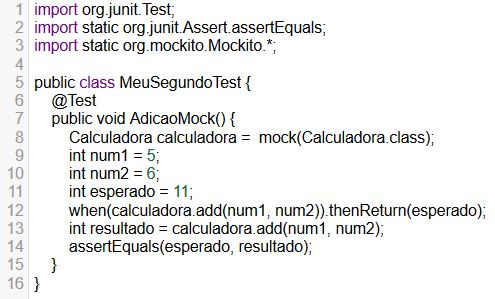
\includegraphics[scale=0.9]{dados/figuras/testeMock.JPG}
	\caption{Teste utilizando Mockito.}
	\label{mockito}
\end{figure}


\begin{itemize}

\item[1]: realiza a importação do pacote de testes \textit{JUnit} onde se encontram as \textit{tags} de anotações e os metodos do \textit{Framework}. 

\item[2]:  é importada a função de \textit{"assertEquals"} do pacote \textit{JUnit}, esta função e responsável por comparar dois valores, o primeiro valor é o valor esperado de uma operação, resultado, ou estado. O segundo valor é o valor resultante da chamada de uma função, classe, ou variável que se deseja testar. 

\item[3]: realiza a importação do pacote \textit{"mockito.Mockito.*"}, onde estão contidos todos os métodos estáticos do pacote e as \textit{tags} de anotações. 


\item[5]: a classe principal \textit{"MeuSegundoTeste"} é aberta. 

\item[6]: é utilizada a anotação \textit{@Test}, esta anotação sinaliza que o método a seguir é um método que deve realizar um teste. 

\item[7]: o método de nome \textit{"AdicaoMock"} é declarado, sendo do tipo \textit{"void"} (sem retorno). 


\item[8]: é instanciado um objeto do tipo \textit{"Calculadora"} na variável \textit{"calculadora"}. Como o objeto que se deseja instanciar se trata de uma interface e não possui comportamento definido, é utilizado a função \textit{“mock”} do pacote \textit{"mockito.Mockito.*"} para que o objeto instanciado possua um comportamento fictício. 

\item[9]: a variável do tipo inteiro \textit{“num1”} é declarada. Ela recebe o valor inteiro "5". 

\item[10]: a variável do tipo inteiro \textit{“num2”} é declarada. Ela recebe o valor inteiro "6".

\item[11]: a variável do tipo inteiro \textit{“esperado”} é declarada. Ela recebe o valor inteiro "11". 

\item[12]: O método \textit{“when().thenReturn()”} do pacote \textit{"mockito.Mockito.*"}  é utilizado para definir o comportamento do objeto \textit{Mock}, o que ele deve fazer em certas situações.
O comando \textit{“when”}  determina qual método deve ser chamado no futuro e quais parâmetros ele deve receber. A ele passamos a função e os parâmetros \textit{"calculadora.add(num1,num2)"}. O \textit{“thenReturn”} diz qual será o valor devolvido quando o método definido no comando \textit{“when”} for chamado. O retorno definimos sendo a variável \textit{“esperado”}.


\item[13]: a variável do tipo inteiro \textit{“resultado”} é declarada. Ela recebe o retorno da função \textit{"calculadora.add(num1,num2)"}. A execução do progama segue com a chamada do metodo  \textit{"add"} realizada pelo objeto \textit{mocado}\footnote{Simula o comportamento de um outro objeto.} instanciado na variável \textit{"calculadora"}. A função \textit{"add"} chamada possui o comportamento definido em \textit{“whem}”  e \textit{“thenReturn"}, recebe dois valores, realiza a soma, e retorna o resultado.

\item[14]: a função importada \textit{assertEquals} é chamada, a ela é passado a variável \textit{“esperado”}, e em seguida a a variável \textit{“resultado}”. A função realiza a comparação entre as variáveis.

\item[15]: o método \textit{"AdicaoMock"} é fechado.

\item[16]: a classe principal é fechada.

\end{itemize}

Caso o retorno da função \textit{"add"} seja um inteiro "11", o mesmo resultado da variável \textit{“esperado”} o resultado do teste será verdadeiro, então logo o teste é aprovado. Caso a função \textit{"add"}  retorne outro valor diferente de um inteiro "11"   o resultado será falso, logo o teste é reprovado. 


    Mais funções do \textit{FrameWork Mockito} serão explorados ao longo deste trabalho.

\section{SPRING FRAMEWORK TEST}

O \textit{Spring Framework} é uma ferramenta que fornece suporte para diversos tipos de aplicações em diferentes etapas do desenvolvimento. Embora testes de unidade busquem testar minuciosamente trechos de código, é importante poder realizar alguns testes de integração sem exigir a implantação do aplicativo em  servidores ou conectá-los com a infraestrutura corporativa \cite{spring}. O \textit{spring-boot-test} é um modlo dedicado somente para testes de integração de aplicativos \textit{Spring Boot}.


Os pacotes de testes contidos na biblioteca do \textit{spring-framework-test} não dependem de servidores de aplicações ou ambientes de execuções. Os testes de implantação são mais lentos do que os testes de unidade, porém, são mais rápidos do que os testes de  interface com Selênio, e equivalentes aos testes remotos que dependem da implantação da aplicação em um servidor. O \textit{Spring Framework Test} fornece suporte a testes de unidade e integração, ele utiliza a orientação por anotações o que permite a criação de testes em vários ambientes, incluindo \textit{JUnit} \cite{spring}. O suporte de testes de integração do \textit{Spring} fornece: 

\begin{itemize}
    \item Gerenciamento de contexto\footnote{Conjunto de dados mínimos usados por uma tarefa que deve ser salvo para permitir uma interrupção da tarefa e a posteriormente a continuação desta tarefa no ponto que ela foi interrompida sem perca de dados.} e cache\footnote{Área de memória onde é mantida uma cópia temporária de dados}, ou seja, o aplicativo é carregado em apenas uma JVM e a partir desta instância todos os testes são executados, o que reduz o tempo de execução dos testes, já que evita que o aplicativo seja carregado toda vez que um teste for executado  \cite{spring}. 


\item Injeção de dependências a partir do contexto de execução de uma aplicação fornece instancias de classes em tempo de execução para outros cenários de testes  \cite{spring}. 


\item Gerenciamento de transações esta funcionalidade garante que as modificações realizadas em base de dados não persistam após a execução de um teste  \cite{spring}. 



\item Classes de suporte para testes de integração o \textit{Spring Framework} fornece várias classes de suporte abstratas que simplificam a criação de testes de integração. Essas classes fornecem ganchos bem definidos na estrutura de teste, bem como variáveis e métodos de instância convenientes  \cite{spring}.

\end{itemize}


% \subsection{Adicionando Spring Boot Test Usando Maven}

% Para a utilização do \textit{Spring Boot Test} basta cria o projeto no site \textit{Spring Initializr} \url{https://start.spring.io/},  ou adicionar as dependências com a ferramenta de gerenciamento de dependências opcional do usuário. A FIGURA \ref{springfig} ilustram a importação do pacote \textit{Spring Boot Starter Test} pela ferramenta de gerenciamento de dependências \textit{Maven}. 

% \begin{figure}[H]
% 	\centering
% 	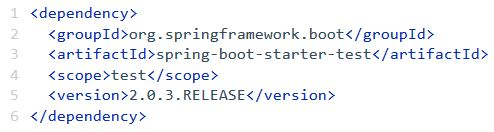
\includegraphics[]{dados/figuras/mavenSpring.JPG}
% 	\caption{Importação do Pacote Spring Boot Starter Test Utilizando Maven.}
% 	Fonte: \cite[https:~//mvnrepository.com/artifact/org.springframework.boot/spring-boot-starter-test/2.0.3.RELEASE]{Maven}
% 	\label{springfig}
% \end{figure}

% A FIGURA \ref{springfig} apresenta a importação do pacote \textit{Spring Boot Starter Test} onde cada linha de código tem a sua seguinte função: 

% \begin{itemize}

% \item[1]: a \textit{tag} \textit{<dependencies>} é aberta, é dentro desta \textit{tag} que cada dependência é definida individualmente, 

% \item[2]: a \textit{tag} \textit{<groupId>} é aberta e fechada, ela é o identificador único do pacote \textit{"org.springframework.boot”} responsável por indicar a coordenada \textit{Mavem} do projeto.

% \item[3]: a \textit{tag} \textit{<artifactId>} é aberta e fechada, ela é geralmente o nome pelo qual o projeto é conhecido \textit{"spring-boot-starter-test"},  ela juntamente com a \textit{tag} \textit{<groupId>} é responsável separar o projeto de todos os outros do repositório central.


% \item[4]: alterações no código geram versões diferentes do mesmo pacotes a \textit{tag} \textit{<version>} \textit{"2.0.3.RELEASE"} indica quais alterações feitas no código e devem ser baixadas.
 
% \item[5]: esta \textit{tag} \textit{<scope>} faz referência ao tipo de trabalho \textit{"test"} que será realizado pelo pacote, e limita a transitividade de um pacote.


% \item[6]: é responsável por fecha a chave de \textit{tags} \textit{<dependency>}.

% \end{itemize}


% Para que a importação seja realizada com sucesso a dependência deve ser declarada em um arquivo de \textit{POM.xml (Project Object Model)} que contem a lista de dependências do projeto, este é a peça fundamental de um projeto Maven \cite{Maven}.


\subsection{Utilizando Spring Boot Test}

O \textit{Spring Framework} fornece um conjunto de anotações específicas do \textit{Spring} que podem ser usadas em testes de unidade e testes de integração em conjunto com o \textit{framework TestContext}.  A FIGURA \ref{springfig2} traz um exemplo do uso de anotações utilizando o spring framework test.

\begin{figure}[H]
	\centering
	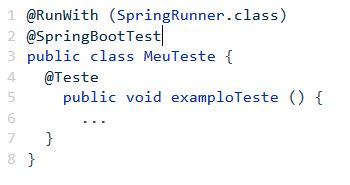
\includegraphics[]{dados/figuras/testeSpring.JPG}
	\caption{Anotações Utilizando o Spring Framework Test.}
	\label{springfig2}
\end{figure}

O trecho de código da FIGURA \ref{springfig2} apresenta a declaração de um teste que utiliza as anotações do \textit{Spring Boot Test}. Cada linha possui a seguinte função:

\begin{itemize}

\item[1]: A anotação \textit{"@RunWith(SpringRunner.class)"}, oferece integração total com o \textit{JUnit} 4 ou superior. Esta anotação define um padrão de configuração personalizado para a classe chamada \cite{spring}. 

\item[2]: O \textit{Spring Boot} fornece a anotação \textit{"@SpringBootTest"}, ela define metadados de nível de classe que são usados para carregar e configurar uma aplicação para testes de interface, ou seja,  carrega as alocações e os recursos necessários para a execução do aplicativo e das classes anotadas usadas no contexto da aplicação \cite{spring}.   

\item[3]: a classe principal \textit{"MeuTeste"} é aberta. 

\item[4]: é utilizada a anotação \textit{"@Test"}, esta anotação sinaliza que o método a seguir é um método que deve realizar um teste. 

\item[5]: o método de nome \textit{"exemploTeste"} é declarado, sendo do tipo \textit{"void"} (sem retorno). 

\item[6]:O corpo do método deve ser implementado aqui.

\item[7]: o método \textit{"exemploTeste"} é fechado.

\item[8]: a classe principal é fechada.

\end{itemize}

O documento completo com todas as anotações, métodos e atributos disponíveis pelo \textit{framework} podem ser encontrados no site oficial do \textit{FrameWork Spring Test} \cite{spring}. Mais funções do \textit{FrameWork} serão explorados ao longo deste trabalho.

